%%%%%%%%%%%%%%%%%%%%%%%%%%%%%%%%%%%%%%%%%
	% Beamer Presentation
	% LaTeX Template
	% Version 1.0 (10/11/12)
	%
	% This template has been downloaded from:
	% http://www.LaTeXTemplates.com
	%
	% License:
	% CC BY-NC-SA 3.0 (http://creativecommons.org/licenses/by-nc-sa/3.0/)
	%
%%%%%%%%%%%%%%%%%%%%%%%%%%%%%%%%%%%%%%%%%

%----------------------------------------------------------------------------------------
	%	PACKAGES AND THEMES
%----------------------------------------------------------------------------------------

\documentclass{beamer}
	
	\mode<presentation> {
	
	% The Beamer class comes with a number of default slide themes
		% which change the colors and layouts of slides. Below this is a list
	% of all the themes, uncomment each in turn to see what they look like.
	
	%\usetheme{default}
		%\usetheme{AnnArbor}
		%\usetheme{Antibes}
		%\usetheme{Bergen}
		%\usetheme{Berkeley}
		%\usetheme{Berlin}
		%\usetheme{Boadilla}
		%\usetheme{CambridgeUS}
		%\usetheme{Copenhagen}
		%\usetheme{Darmstadt}
		%\usetheme{Dresden}
		%\usetheme{Frankfurt}
		%\usetheme{Goettingen}
		%\usetheme{Hannover}
		%\usetheme{Ilmenau}
		%\usetheme{JuanLesPins}
	%\usetheme{Luebeck}
	\usetheme{Madrid}
	%\usetheme{Malmoe}
		%\usetheme{Marburg}
		%\usetheme{Montpellier}
		%\usetheme{PaloAlto}
		%\usetheme{Pittsburgh}
		%\usetheme{Rochester}
		%\usetheme{Singapore}
		%\usetheme{Szeged}
	%\usetheme{Warsaw}
	
	% As well as themes, the Beamer class has a number of color themes
		% for any slide theme. Uncomment each of these in turn to see how it
	% changes the colors of your current slide theme.
	
	%\usecolortheme{albatross}
		%\usecolortheme{beaver}
		%\usecolortheme{beetle}
		%\usecolortheme{crane}
		%\usecolortheme{dolphin}
		%\usecolortheme{dove}
		%\usecolortheme{fly}
		%\usecolortheme{lily}
		%\usecolortheme{orchid}
		%\usecolortheme{rose}
		%\usecolortheme{seagull}
		%\usecolortheme{seahorse}
		%\usecolortheme{whale}
	%\usecolortheme{wolverine}
	
	%\setbeamertemplate{footline} % To remove the footer line in all slides uncomment this line
	%\setbeamertemplate{footline}[page number] % To replace the footer line in all slides with a simple slide count uncomment this line
	
	\setbeamertemplate{navigation symbols}{} % To remove the navigation symbols from the bottom of all slides uncomment this line
	}
	
	\usepackage{graphicx} % Allows including images
	\usepackage{booktabs} % Allows the use of \toprule, \midrule and \bottomrule in tables
	
	\usepackage{amsmath}
	
	\usepackage{accents}
	\usepackage{tikz}
	\usepackage{hyperref}
	\hypersetup{
	colorlinks=true,
	linkcolor=blue,
	filecolor=magenta,      
	urlcolor=blue,
	}
	
	%----------------------------------------------------------------------------------------
		%	TITLE PAGE
	%----------------------------------------------------------------------------------------
	
	\title[Anderson Acceleration]{Anderson Acceleration for Fixed-Point Iterations} 
		\subtitle {Project in Numerical Analysis of Partial Differential Equations}
		\author[Martino Ischia]{Martino Ischia\\ \footnotesize{Supervisor: Prof. Formaggia}} 
		\institute[]
		{
		Politecnico di Milano
		}
		\date{May 28, 2020} 
		
		\begin{document}
			
			\begin{frame}
				\titlepage 
			\end{frame}
				
				\begin{frame}
					\frametitle{Context}
					\begin{itemize}
						\item Fixed-point iterations, looking for $x\in\mathbb{R}^n$ such that $x=g(x)$
						$$x_{k+1} = g(x_k)$$
						\item The case of linear systems:
						$$x_{k+1} = g(x_k) = A x_k + b$$
						\item Krylov based methods are usually preferred for large   systems
					\end{itemize}
				\end{frame}
				
				%------------------------------------------------
				
				\begin{frame}{Context}
					
					\begin{itemize}
						\item The problem can be written equivalently as the equation
						$$ f(x) = x - g(x) = 0 $$
						\item In the case where $g$ is nonlinear, \textbf{Newton method} typically shows quadratic convergence;
						\item Fixed-point form of the problem has typically linear convergence (often unacceptably slow for large systems)
						\item  Acceleration strategies
					\end{itemize}    
				\end{frame}
				
				
				\begin{frame}{Anderson Acceleration \hypersetup{linkcolor=white}\cite{p5}\hypersetup{linkcolor=blue}}
					
					Given $x_0$ and $m \geq 1$\\
					Set $x_1 = g(x_0)$\\
					For $k = 1, 2, ...$\\
					\hspace*{16pt} Set $m_k = min\{m, k\}$\\
					\hspace*{20pt}Set $F_k = (f_{k-m_k}, ... , f_k)$, where $f_i = g(x_i)-x_{i}$\\
					\hspace*{20pt}Determine $\alpha^{(k)} = (\alpha^{(k)}
					_0 , ..., \alpha^{(k)}_{m_k} )^T$, subject to\\ \hspace*{20pt}$\sum^{m_k}_{i=0} {\alpha_i = 1}$, that solves
					$$\min_{\alpha=(\alpha_0,...,\alpha_{m_k} )^T} \|F_k \alpha\|_2$$\\
					\hspace*{20pt}Set $x_{k+1} =\sum^{m_k}
					_{i=0} {\alpha_i^{(k)} g(x_{k-m_{k}+i})}$    
				\end{frame}
				
				\begin{frame}{Properties}
					% In the linear case $g(x_k) = A x + b$,\\
						% since $\sum^{m_k}_{i=0} {\alpha_i = 1}$,
						% $$x_{k+1} =\sum^{m_k}
						% _{i=0} {\alpha_i^{(k)} g(x_{k-m_{k}+i})} = \sum^{m_k}
					% _{i=0} {g(\alpha_i^{(k)}x_{k-m_{k}+i})} $$
					\begin{itemize}
						\item In the linear case, when $m = \infty$, GMRES solves the same least squares problem and $x_{k+1}^A = g(x_k^{GMRES})$
						\item It is a particular case of multisecant updating method \cite{p3}
					\end{itemize}
					
					
				\end{frame}
				
				
				\begin{frame}{Anderson Jacobi and Alternating Anderson Jacobi}
					\begin{itemize}
						\item Applying Anderson algorithm to the Jacobi method, already good results are achieved;
						\item Another possibility is to alternate a number of Jacobi iterations to an Anderson iteration. Great for parallelization and has showed great results \cite{p2}
					\end{itemize}
					
					\begin{figure}
						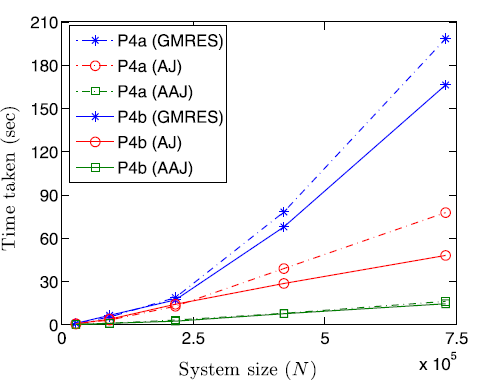
\includegraphics[scale= 0.5]{AAJ.png}
						\caption{Poisson problem \cite{p2}}
						% \centering
					\end{figure}
				\end{frame}
				
				\begin{frame}{Goal of the Project}
					\begin{itemize}
						\item Develop a C++ interface for generic nonlinear problems and generic accelerators
						\item Performance tests for problems coming from discretization of PDEs
						
						
					\end{itemize}
					
					
				\end{frame}
				
				
			%------------------------------------------------
			\section{References}
				%------------------------------------------------
				
				\begin{frame}
					\frametitle{References}
					\fontsize{6pt}{7.2}\selectfont
					\begin{thebibliography}{99}
						\bibitem[Walker \& Ni, 2011]{p1} Walker, Homer \& Ni, Peng. (2011). Anderson Acceleration for Fixed-Point Iterations. SIAM J. Numerical Analysis. 49. 1715-1735. 10.2307/23074353.
						\bibitem[Pratapa \& al., 2015]{p2}Pratapa, Phanisri \& Suryanarayana, Phanish \& Pask, John. (2015). Anderson acceleration of the Jacobi iterative method: An efficient alternative to Krylov methods for large, sparse linear systems. Journal of Computational Physics. 306. 10.1016/j.jcp.2015.11.018.
						\bibitem[Fang \& Saad 2009]{p3}Fang, Haw-ren \& Saad, Yousef. (2009). Two classes of multisecant methods for nonlinear acceleration. Numerical Linear Algebra with Applications. 16. 197 - 221. 10.1002/nla.617.
						\bibitem[Ramière \& Helfer 2015]{p4}Ramière, Isabelle \& Helfer, Thomas. (2015). Iterative residual-based vector methods to accelerate fixed point iterations. Computers \& Mathematics with Applications. 70. 10.1016/j.camwa.2015.08.025.
						\bibitem[Anderson, 1965]{p5}Anderson, Donald. (1965). Iterative Procedures for Nonlinear Integral Equations. J. ACM. 12. 547-560. 10.1145/321296.321305.
					\end{thebibliography}
				\end{frame}
			
			
			%------------------------------------------------
			
			%----------------------------------------------------------------------------------------
			
			\end{document} 
						